% prefazione


\begin{figure}[h]
	\centering
	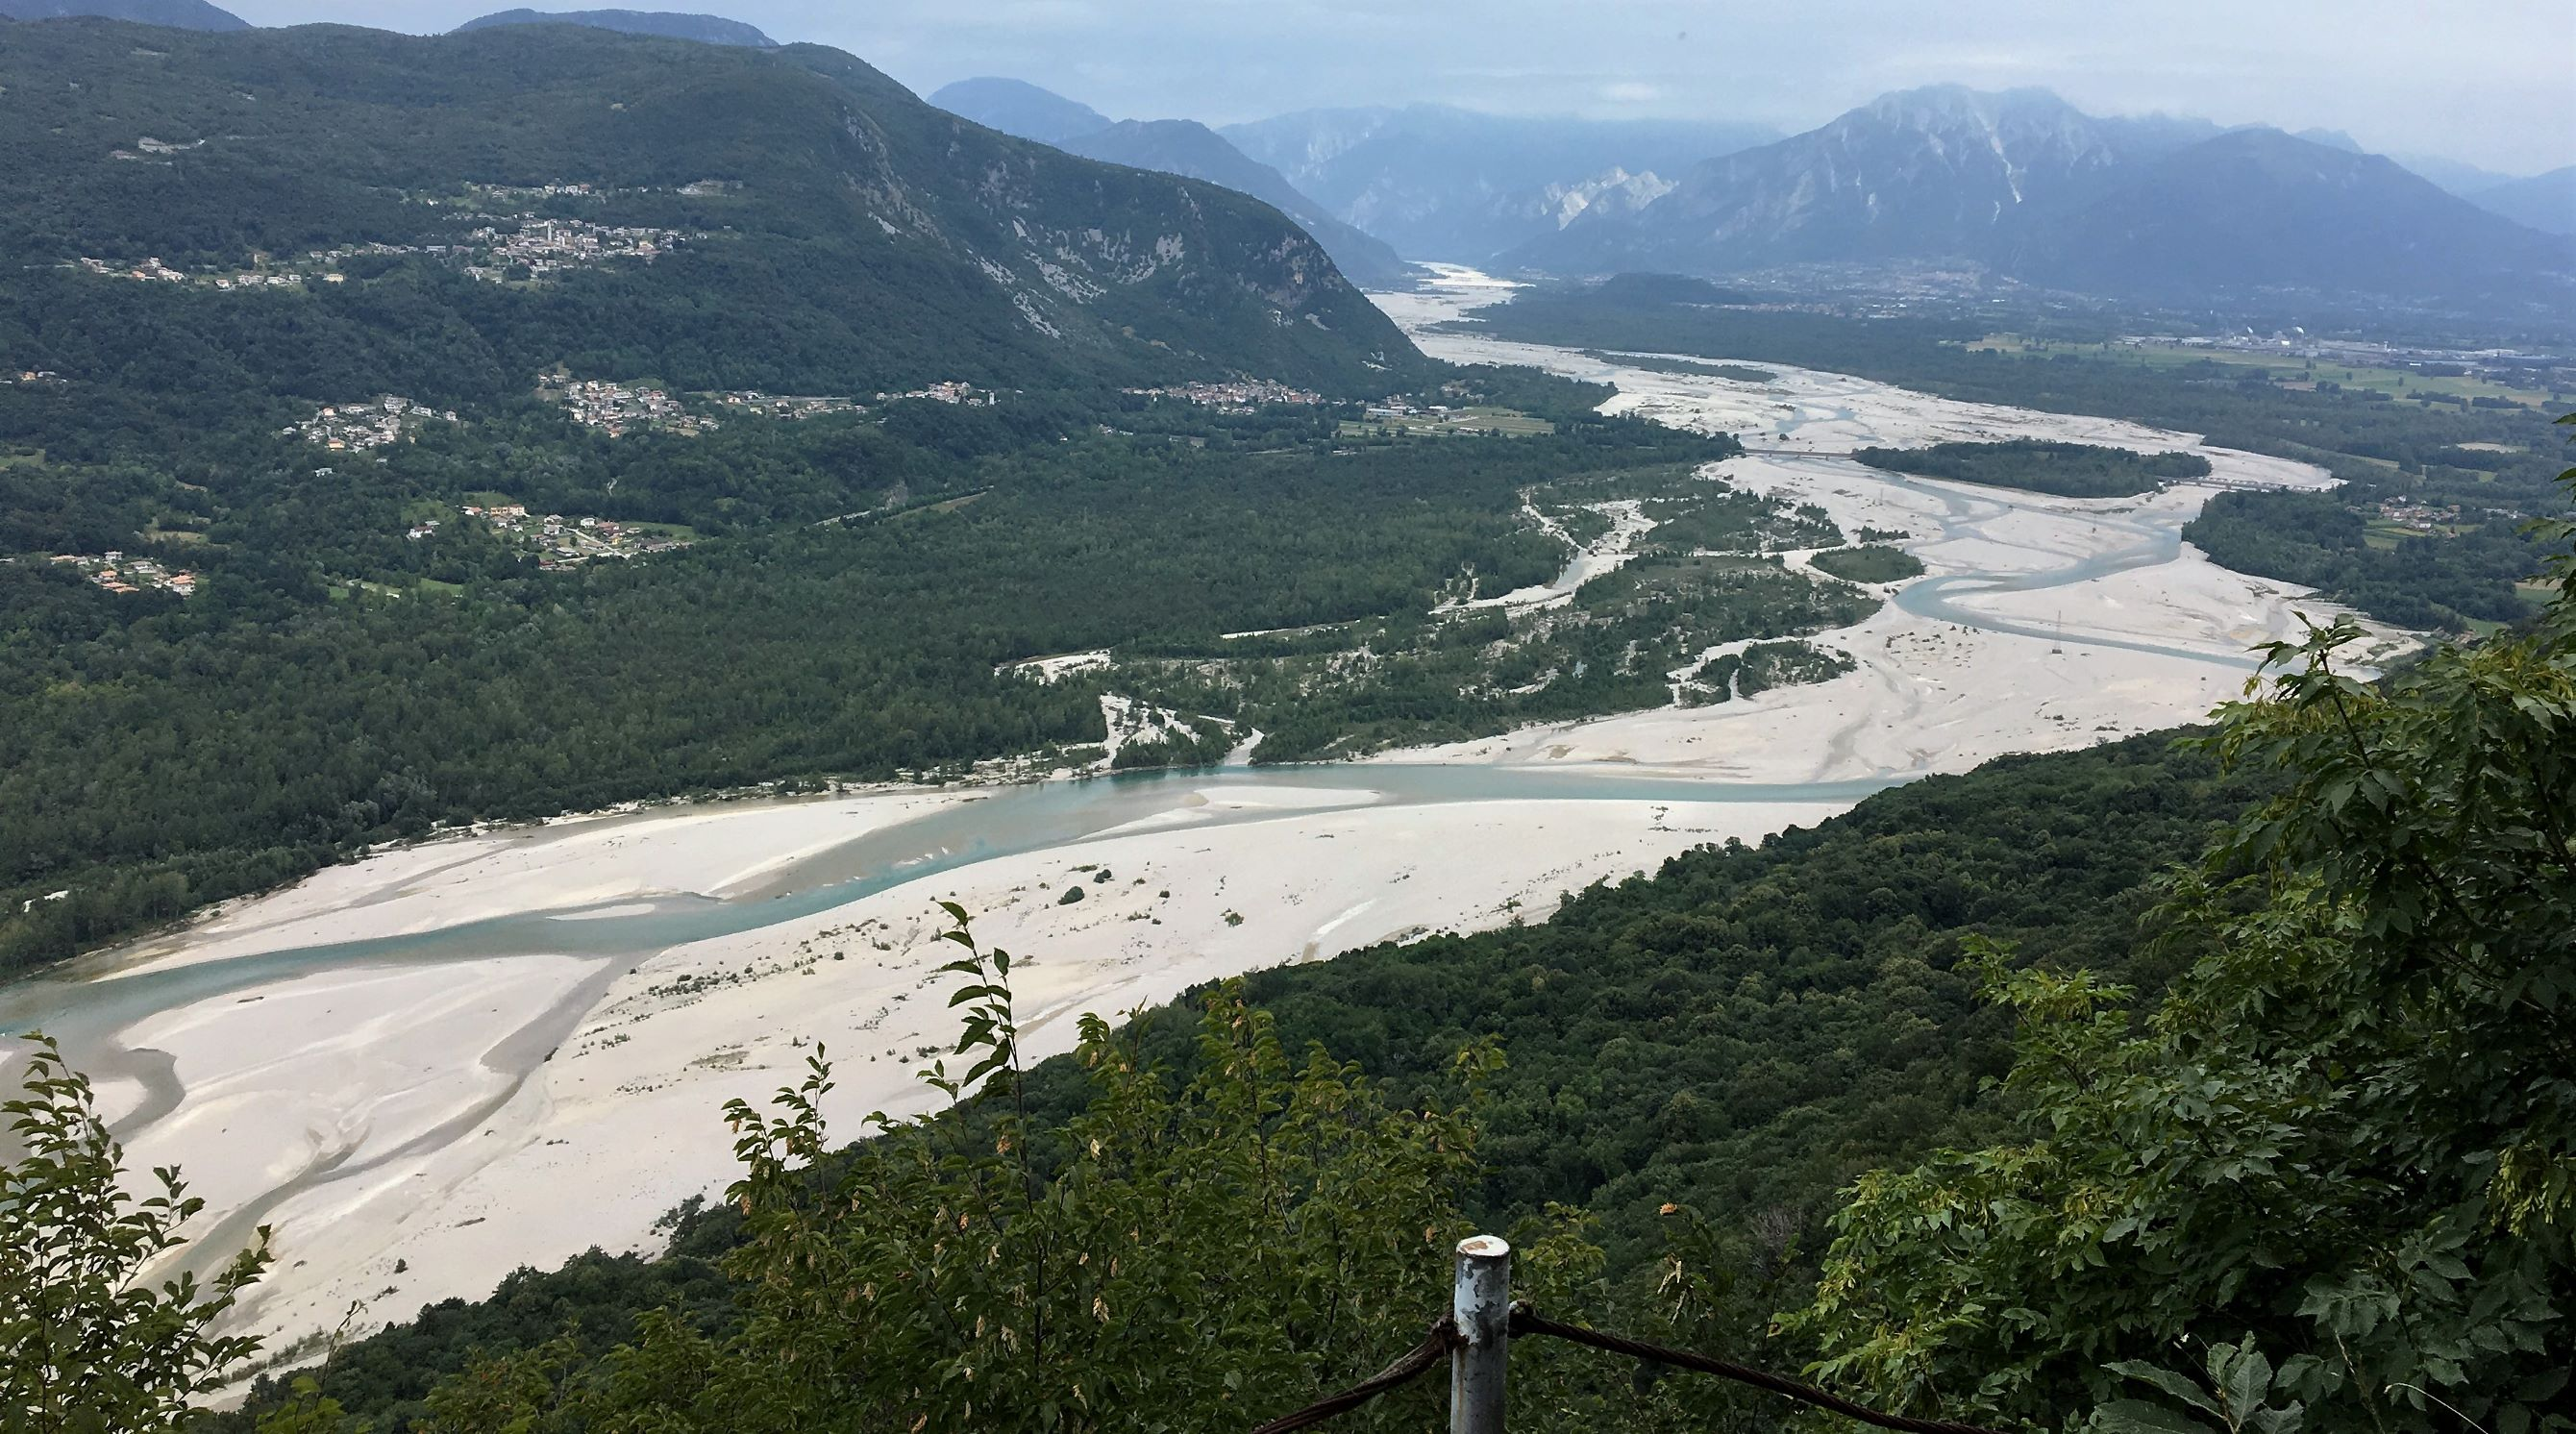
\includegraphics[width=\textwidth]{files/foto_flagogna.jpg}
	\caption[foto di un tratto del Tagliamento ripreso dal monte di Ragogna]{foto di un tratto del Tagliamento ripreso dal monte di Ragogna~(UD); l'acqua scorre da destra verso sinistra.
	}
	\label{fig:foto-ragogna}
\end{figure}



Questa prima figura mostra un fiume che scorre, libero, su un letto di ghiaia che forse pare essere decisamente più largo di quanto gli basterebbe. 
Dove sono gli argini? Il fiume può spostarsi? 
%
In mezzo alla figura si vedono numerose isole divise dal resto della vegetazione da canali abbandonati in ghiaia e sabbia. 
Come si formano? Rimangono inalterate al passare degli anni? 
%
Poco più in basso, dall'altra parte del canale, si intravedono degli arbusti proprio sulla ghiaia. 
Cresceranno fino a formare un'isola tanto vegetata quanto le vicine sue sorelle più a monte? O saranno spazzati via durante la prossima piena?

\medskip
Queste e altre cose si possono leggere da questa foto, così come da quella successiva. Tutte le domande hanno un carattere dinamico più o meno evidente: la loro risposta non la si può ottenere osservando una foto, che è statica, ma una sequenza di istanti successivi quale può essere un filmato.
Come racconta un professore, occorre sincronizzare i nostri orologi con quello del fiume; non solo, bisogna anche che indossiamo gli occhiali giusti per guardare i fenomeni alla scala in cui si possono vedere. Chi mai trarrebbe conclusioni effettive sulla vita di un albero se guardasse solo la sua foglia per pochi secondi, o se lo confrontasse su due immagini satellitari acquisite a distanza di diversi decenni?

\begin{figure}
	\centering
	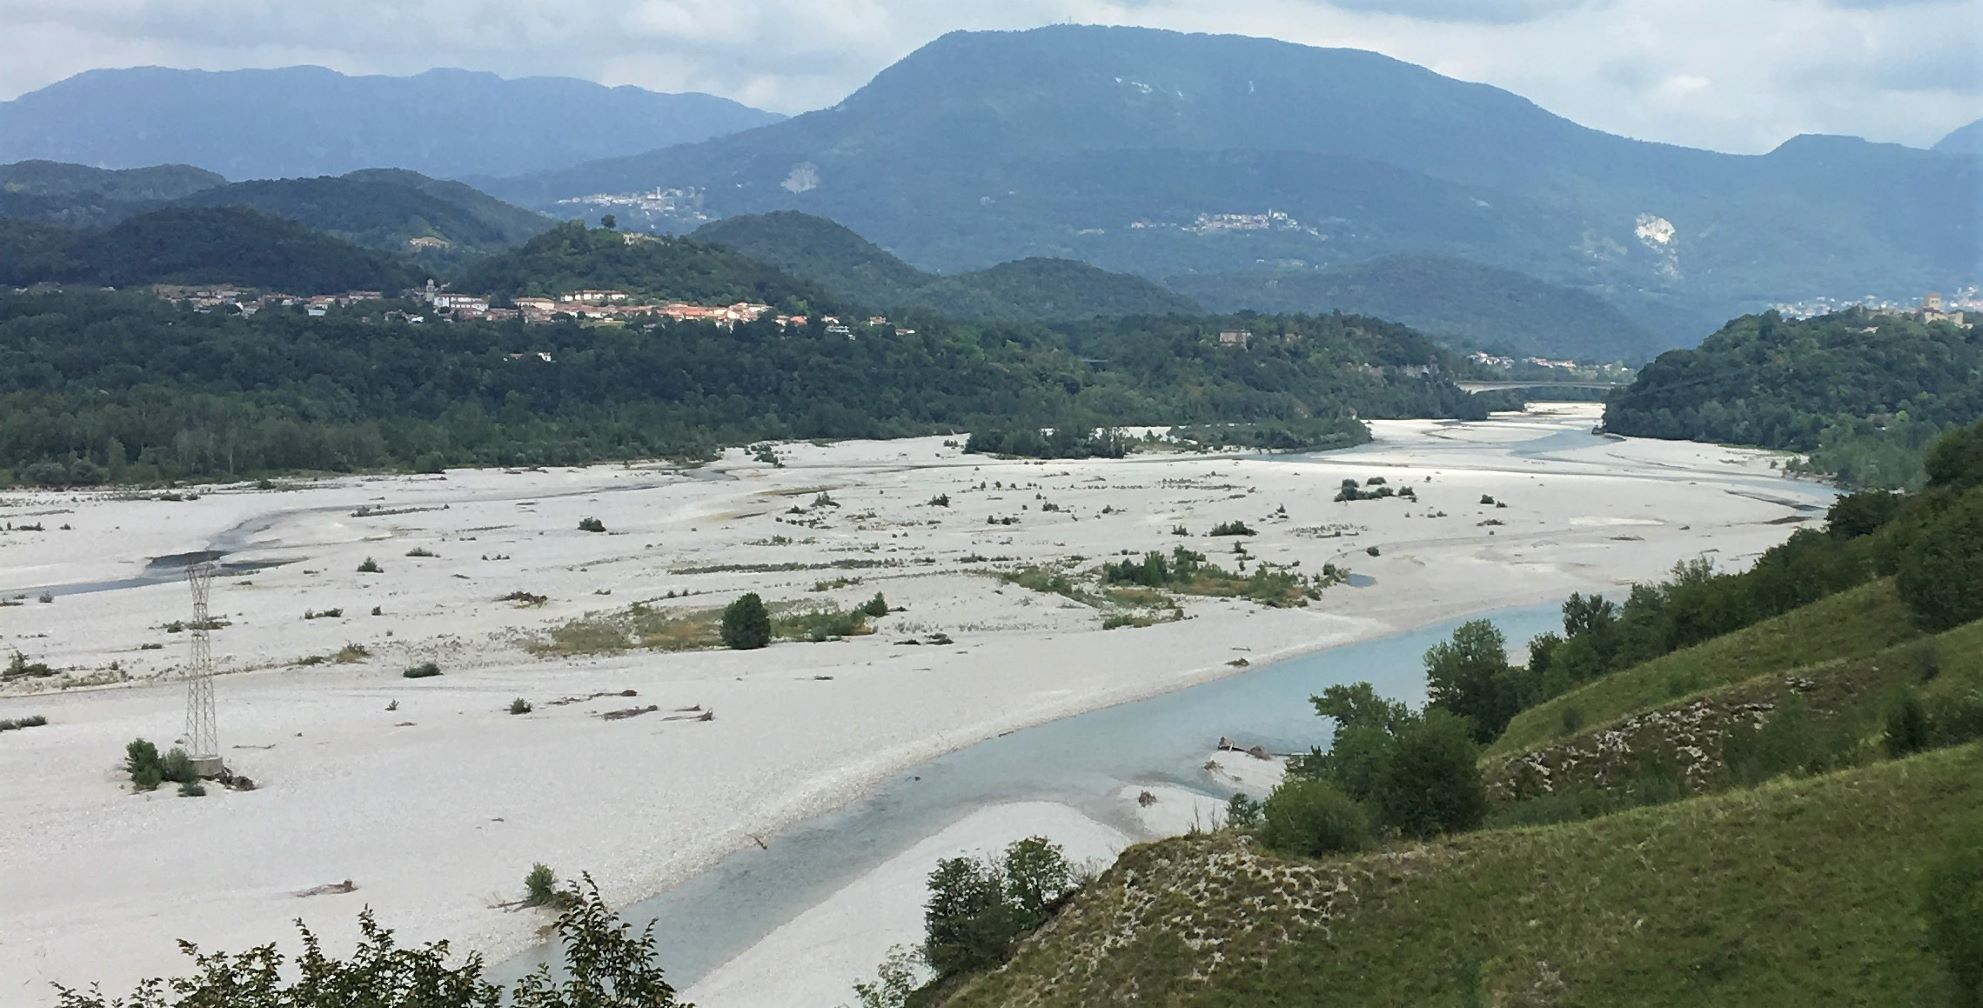
\includegraphics[width=\textwidth]{files/foto_terrazzo_valle_pinzano.jpg}
	\caption[foto di un tratto del Tagliamento ripreso dal terrazzo presso Aonedis~(UD)]{foto di un tratto del Tagliamento ripreso dal terrazzo presso Aonedis~(UD); l'acqua scorre da destra verso sinistra. 
	}
	\label{fig:foto-pinzano}
\end{figure}


Tra tutti i fiumi che ci sono nel nostro bel Paese, pochi di loro sono rimasti in condizioni “naturali”; l'alterazione ha apportato modifiche o ridotto l'entità dei processi che avevano luogo prima dell'intervento dell'uomo. 
Ad esempio, la costruzione di una diga a monte di un fiume può aver indotto nel corso degli anni un restringimento del suo alveo e ad un cambiamento della sua morfologia.
Ma in questo caso siamo fortunati: il Tagliamento può essere considerato un fiume alpino allo stato praticamente naturale.

Le domande che ho posto all'inizio nascono dalla curiosità che si può avere quando, dopo mesi di studio dei fenomeni che naturalmente avvengono nei fiumi, si incontra un fiume dove questi fenomeni possono accadere per davvero. Le domande trovano una risposta reale, comprovata da ciò che si vede quando si cammina sulla ghiaia, in mezzo alle isole, nei canali, e quando ci si tuffa nelle loro confluenze.

\medskip
La \cref{fig:confronto-imm-prefaz} mostra diversi processi che avvengono in questo fiume; questi, inutile ripeterlo, diventano apprezzabili solo dopo aver indossato gli occhiali e l'orologio giusti, cioè osservando da un'altezza di poche centinaia di metri da terra e confrontando immagini distanti pochi mesi. Ecco un'anteprima:
\begin{itemize}
	\item si vede subito che i canali migrano e si spostano durante gli anni; 
		difatti durante le piene più importanti tutto l'alveo si riempie di acqua e il fondo viene rimodellato;
	\item lo spostamento dei canali porta questi ad erodere lateralmente le isole, come si vede per l'isola in alto a sinistra in alveo; 
		il fiume quindi potrà trasportare non solo il materiale presente sul fondo, ma anche quello che erode dalle isole, sia ghiaia e sabbia che alberi;
	\item le isole possono espandersi da piccoli nuclei fino a unirsi, diventare più fitte e più resistenti all'erosione da parte dell'acqua, come si vede per la grande isola al centro della \cref{fig:confronto-imm-prefaz};
	\item l'erosione non risparmia le sponde, come si vede per la sponda a sinistra (in destra idrografica se si osserva il verso della corrente) la quale arretra di più di \SI{100}{\m} a causa delle piene che si susseguono nei tre anni di osservazione;
	\item l'erosione di isole e sponda produce moltissimo materiale legnoso (alberi sradicati) il quale si deposita poco più a valle della zona di erosione, come testimoniano i numerosi puntini scuri presenti sull'alveo asciutto; 
		se le condizioni sono adatte e se le piante sono in grado, è possibile che dai tronchi depositati crescano nuovi rami e radici; 
		questi tronchi diventano i nuclei di formazione di future isole;
	\item lo spostamento dei canali è limitato dalla presenza delle isole, che si configurano come ostacolo per la corrente anche durante le piene;
		difatti è difficile che il canale si possa spostare dove c'è l'isola in alto a destra, a meno che non riesca ad eroderla.
\end{itemize}

\begin{figure}
	\centering
	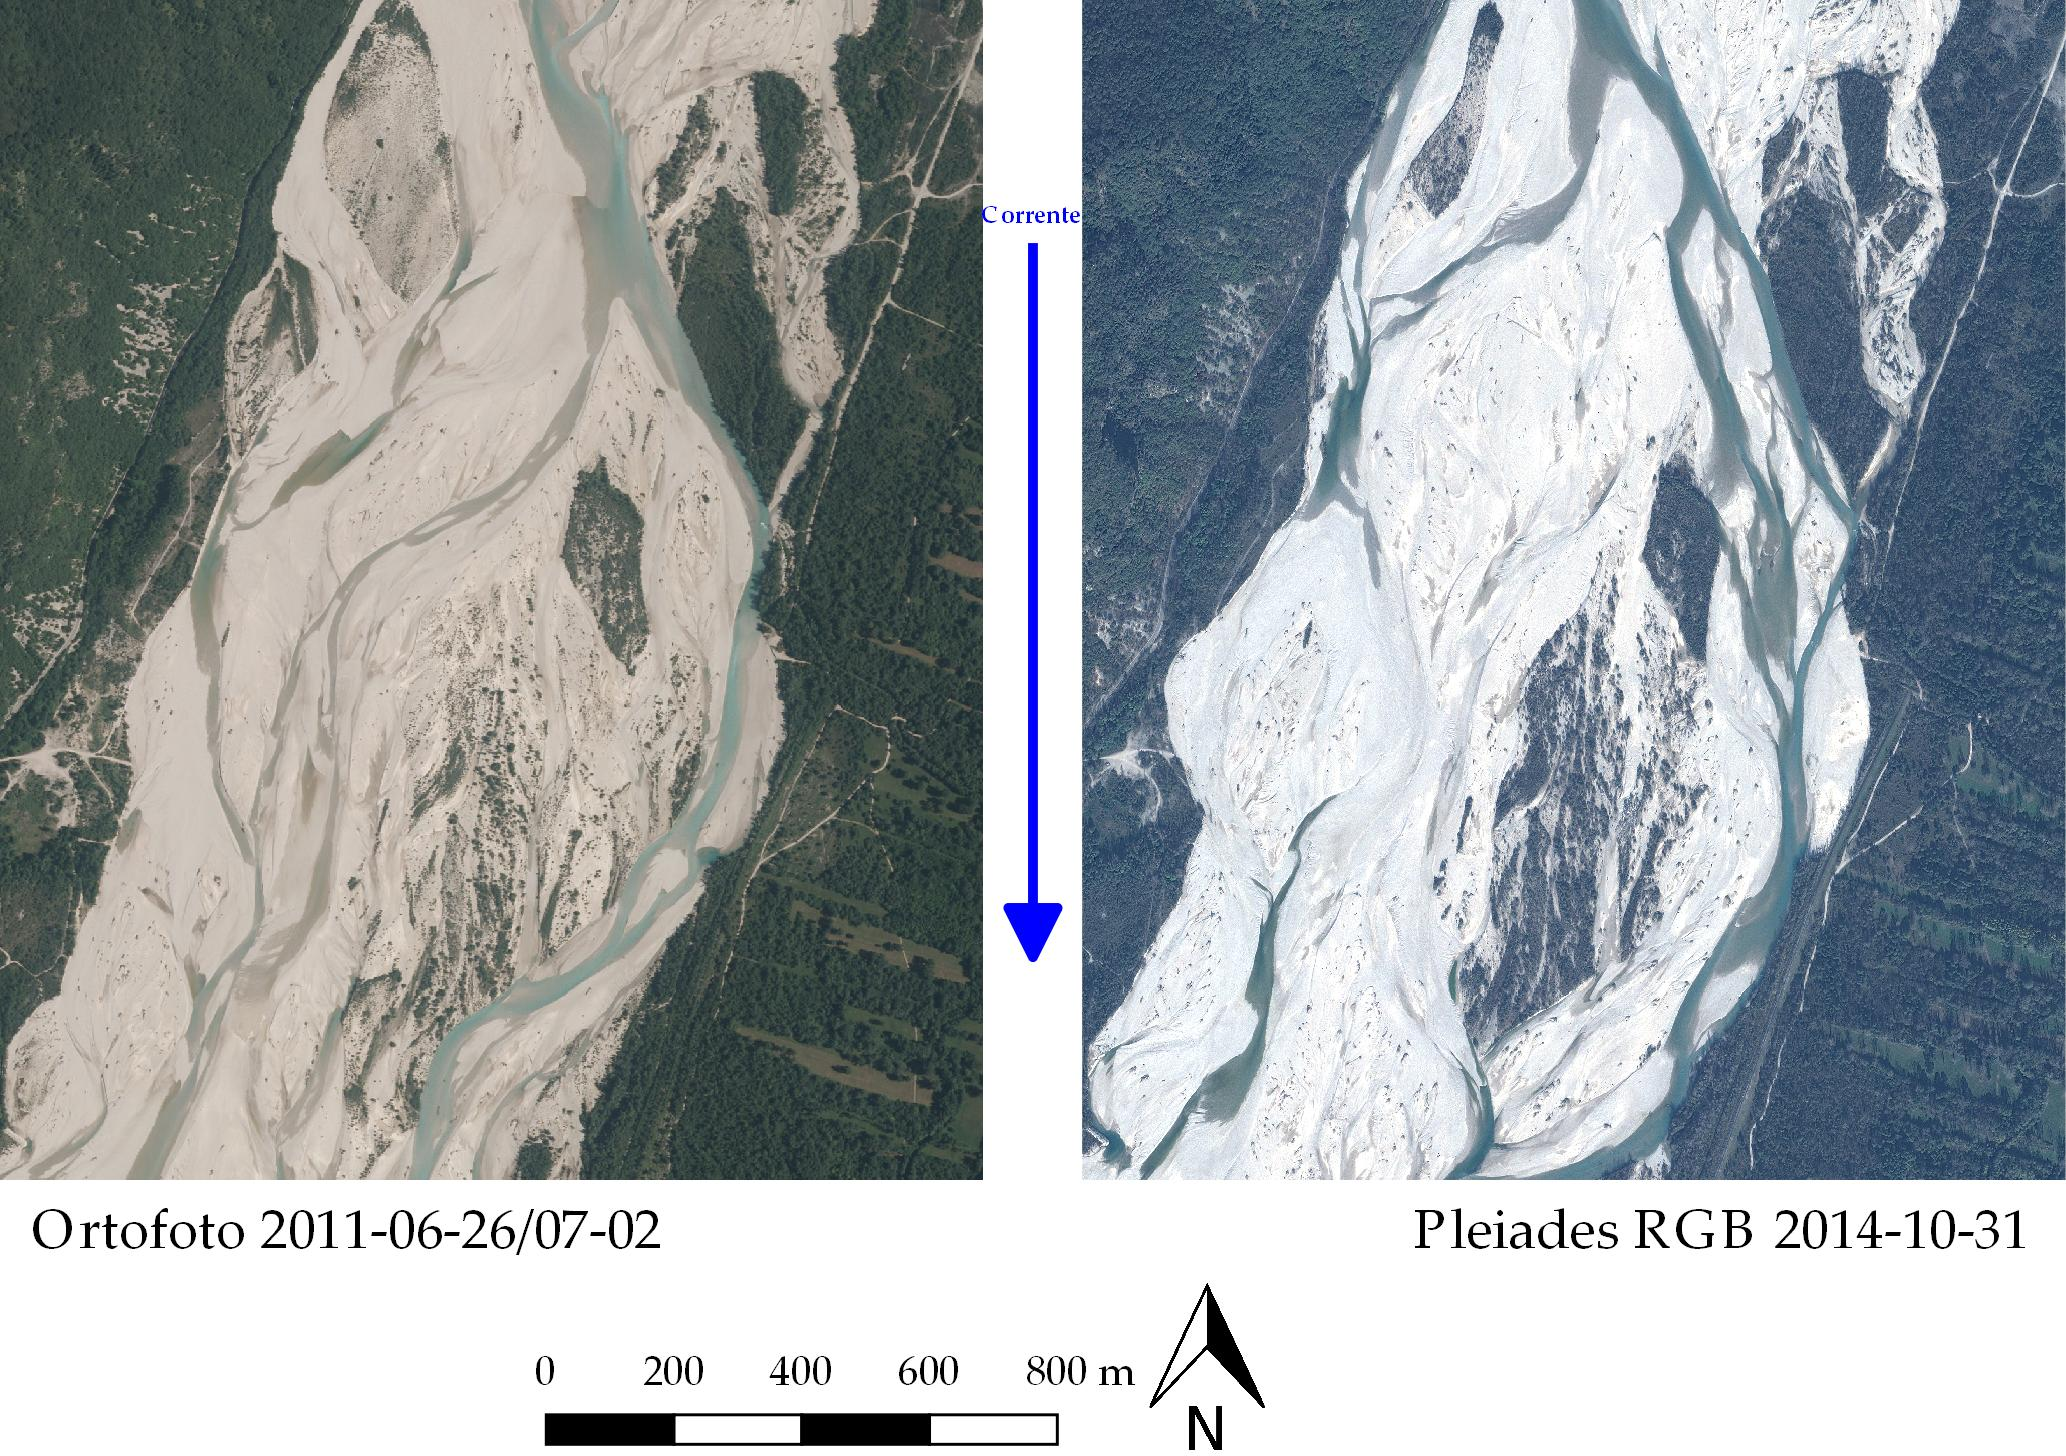
\includegraphics[width=\textwidth]{files/confronto_immagini_erosione_isole.jpeg}
	\caption[immagini di un tratto posto circa \SI{2}{\kilo\m} a monte del ponte di Cornino]{immagini di un tratto posto circa \SI{2}{\kilo\m} a monte del ponte di Cornino~(UD); l'ortofoto proviene dal Portale Cartografico Nazionale del Ministero dell'Ambiente.
	}
	\label{fig:confronto-imm-prefaz}
\end{figure}


Quante cose si possono osservare! In un fiume siffatto sono presenti numerosi altri fenomeni anche a scale diverse.
Ho raccontato quelli che mi interessano particolarmente e che sono oggetto di questa tesi: le dinamiche della vegetazione sulle isole e le dinamiche del legno depositato in alveo.

\medskip
A pensarci bene, non è sorprendente che in un sistema naturale la componente biologica influenzi fortemente quella fisica: i boschi consolidano i pendii e le foreste determinano la forma meandriforme di molti fiumi. Attraverso altri esempi ci si può convincere che le isole vegetate e i tronchi che rigettano in arbusti possano esercitare effetti su un fiume e viceversa. 
\\
E riflettendo ancora non è difficile osservare che queste interazioni solitamente possono indurre effetti positivi sia per l'ambiente che per l'essere umano: per portare qualche esempio, nel caso del Tagliamento si parla di biodiversità data da un mosaico in continuo cambiamento di ambienti diversi, di purificazione dell'acqua, del mantenimento di un microclima particolarmente adatto alla stagionatura del prosciutto di San Daniele (prodotto nell'omonimo paese poco distante) e di un luogo molto adatto per la ricreazione da parte delle persone (\cref{fig:bagnanti}).

Da questi fatti muovo i primi passi verso l'approfondimento dei processi che portano un fiume a modificarsi di continuo assieme all'ambiente in cui si colloca.


\begin{figure}[hb]
	\centering
	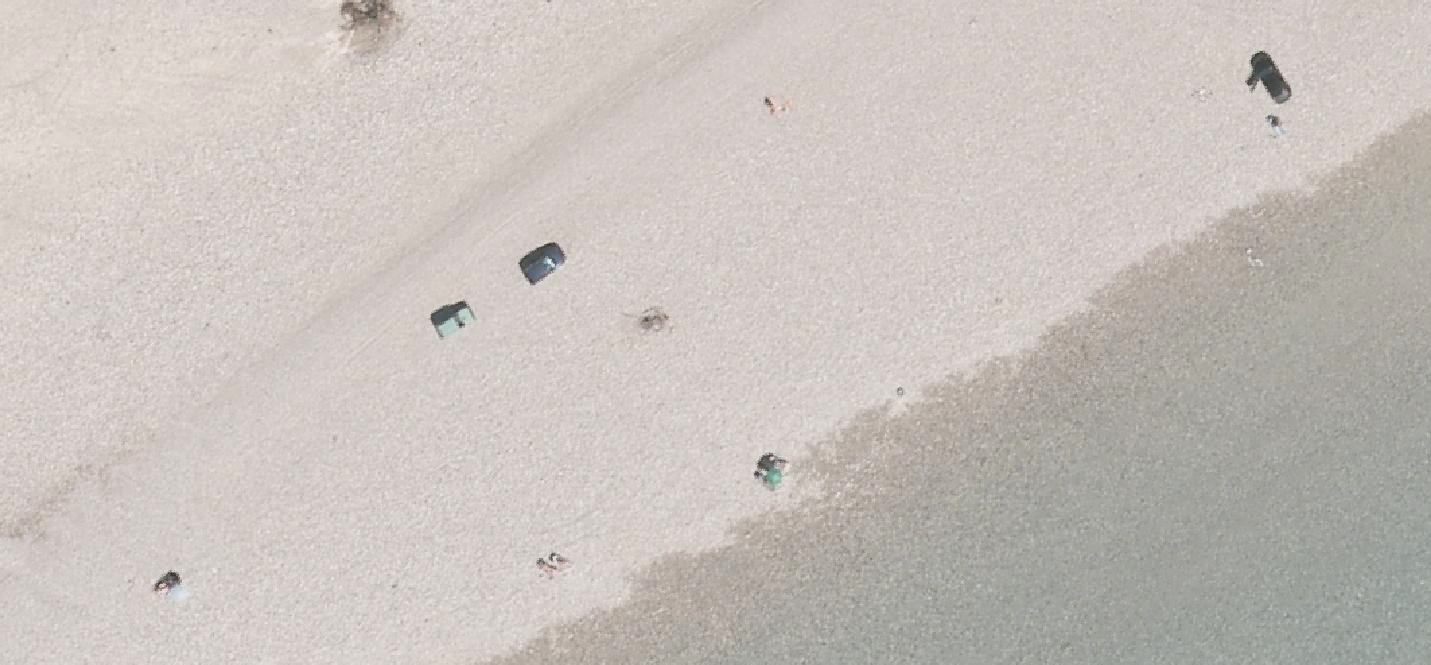
\includegraphics[width=\textwidth]{files/bagnanti.jpeg}
	\caption[bagnanti accanto ad un canale]{bagnanti accanto ad un canale ripresi con una immagine area del~2011, cortesemente fornita da Nicola Surian (Università degli studi di Padova).}
	\label{fig:bagnanti}
\end{figure}


